\section{Pruebas de rango de medición mínimo}
\begin{figure}[H]
	\centering
	\begin{subfigure}{0.6\textwidth}
		\centering
		\includegraphics[width=0.5\linewidth]{disposicion_lidar5.jpeg}
		\caption{Disposición del sensor FHL-LD20 dentro del entorno circular: 7 cm de radio}
		\label{disposicion_lidar5}
		\vspace{1em}
	\end{subfigure}
	\begin{subfigure}{0.45\textwidth}
		\centering
		\includegraphics[width=0.7\linewidth]{try_7cm_r.png}
		\caption{Reconstrucción en coordenadas polares de tres revoluciones completas de lectura en entorno circular: 7 cm de radio}
		\label{try_7cm_r}
	\end{subfigure}
	\hspace{1em}
	\begin{subfigure}{0.45\textwidth}
		\centering
		\includegraphics[width=0.7\linewidth]{try_7cm_r_car.png}
		\caption{Reconstrucción en coordenadas cartesianas de tres revoluciones completas de lectura en entorno circular: 7 cm de radio}
		\label{try_7cm_r_car}
	\end{subfigure}
	\caption{Reconstrucciones vacías de tres revoluciones completas de lectura en entorno circular: 7 cm de radio}
	\label{fig: reconstrucciones_vacías_7}
\end{figure}

\begin{figure}[H]
	\centering
	\begin{subfigure}{0.6\textwidth}
		\centering
		\includegraphics[width=0.6\linewidth]{disposicion_lidar6.jpeg}
		\caption{Disposición del sensor FHL-LD20 dentro del entorno circular: 8 cm de radio}
		\label{disposicion_lidar6}
		\vspace{1em}
	\end{subfigure}
	\begin{subfigure}{0.45\textwidth}
		\centering
		\includegraphics[width=0.8\linewidth]{try_8cm_r.png}
		\caption{Reconstrucción en coordenadas polares de tres revoluciones completas de lectura en entorno circular: 8 cm de radio}
		\label{try_8cm_r}
	\end{subfigure}
	\hspace{1em}
	\begin{subfigure}{0.45\textwidth}
		\centering
		\includegraphics[width=0.8\linewidth]{try_8cm_r_car.png}
		\caption{Reconstrucción en coordenadas cartesianas de tres revoluciones completas de lectura en entorno circular: 8 cm de radio}
		\label{try_8cm_r_car}
	\end{subfigure}
	\caption{Reconstrucciones vacías de tres revoluciones completas de lectura en entorno circular: 8 cm de radio}
	\label{fig: reconstrucciones_vacías_8}
\end{figure}


\begin{figure}[H]
	\centering
	\begin{subfigure}{0.6\textwidth}
		\centering
		\includegraphics[width=0.6\linewidth]{disposicion_lidar7.jpeg}
		\caption{Disposición del sensor FHL-LD20 dentro del entorno circular: 9 cm de radio}
		\label{disposicion_lidar6}
		\vspace{1em}
	\end{subfigure}
	\begin{subfigure}{0.45\textwidth}
		\centering
		\includegraphics[width=0.8\linewidth]{try_9cm_r.png}
		\caption{Reconstrucción en coordenadas polares de tres revoluciones completas de lectura en entorno circular: 9 cm de radio}
		\label{try_9cm_r}
	\end{subfigure}
	\hspace{1em}
	\begin{subfigure}{0.45\textwidth}
		\centering
		\includegraphics[width=0.8\linewidth]{try_9cm_r_car.png}
		\caption{Reconstrucción en coordenadas cartesianas de tres revoluciones completas de lectura en entorno circular: 9 cm de radio}
		\label{try_9cm_r_car}
	\end{subfigure}
	\caption{Reconstrucciones vacías de tres revoluciones completas de lectura en entorno circular: 9 cm de radio}
	\label{fig: reconstrucciones_vacías_9}
\end{figure}

\section{Pruebas para la estimación de la varianza asociada a las mediciones de distancia del sensor}
\begin{figure}[H]
	\centering
	\begin{subfigure}{\textwidth}
		\centering
		\makebox[\textwidth]{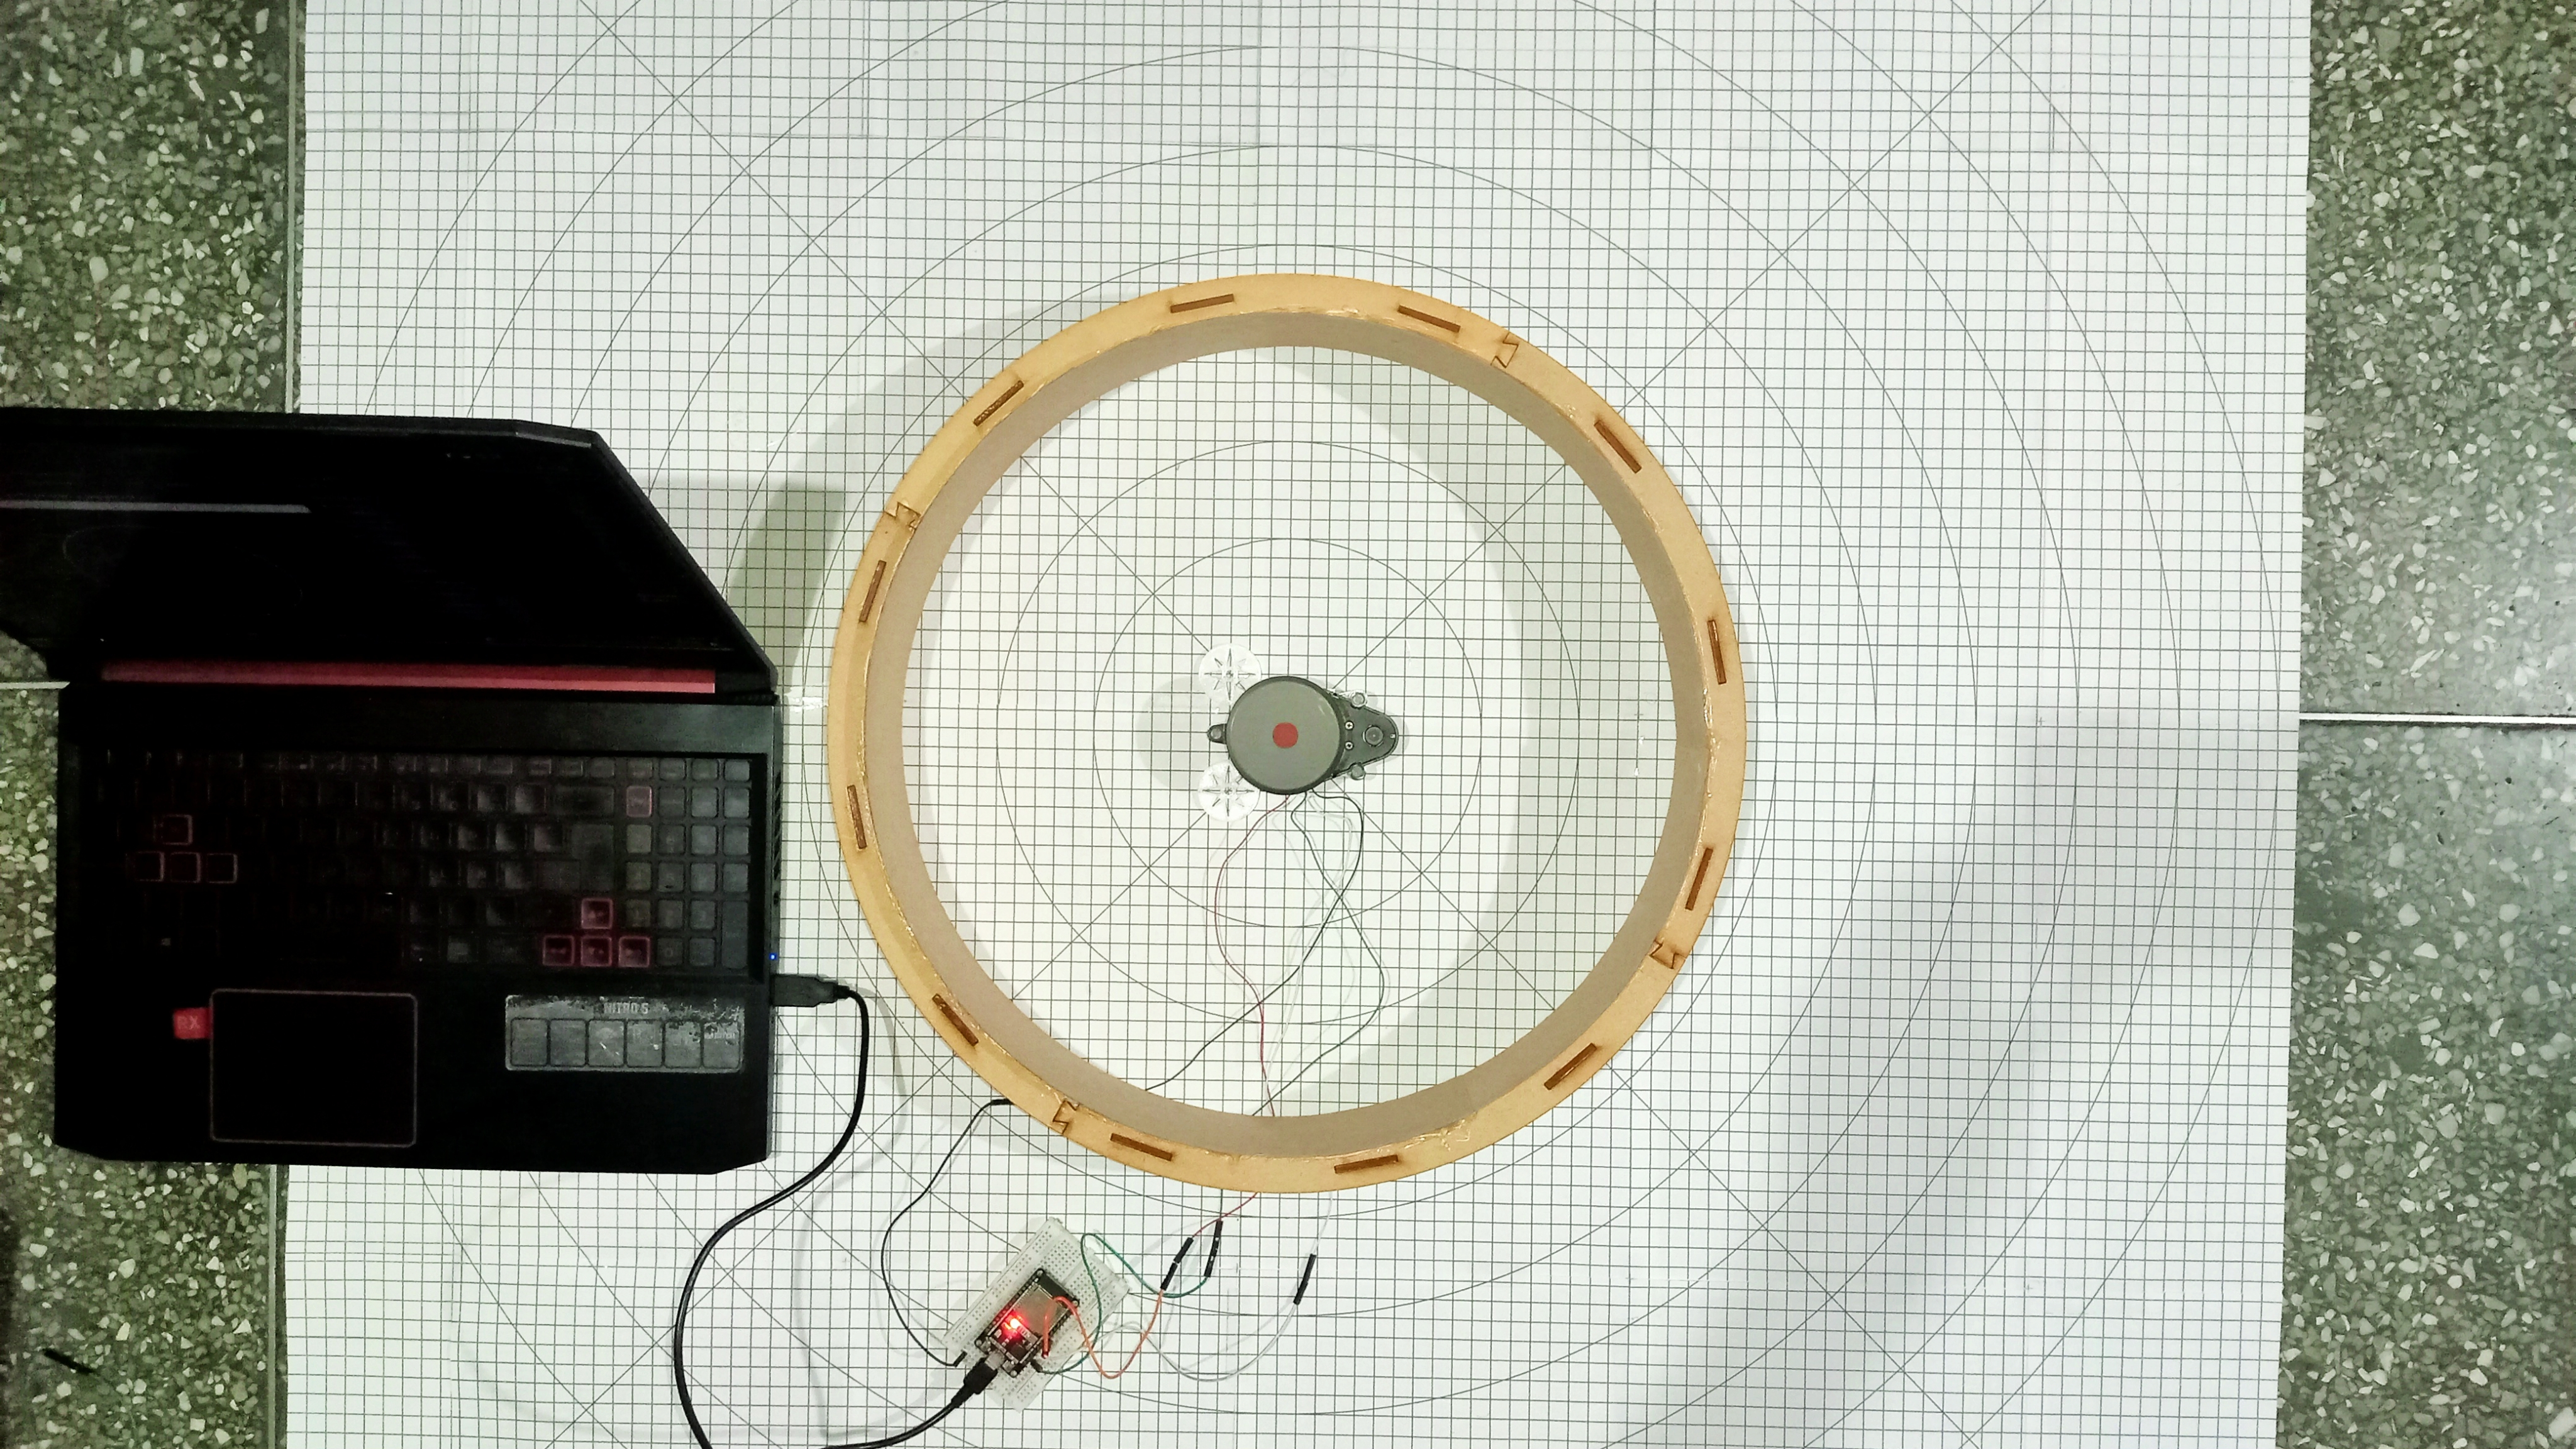
\includegraphics[width=0.6\linewidth]{disposicion_lidar_var_dist2.jpg}}
		\caption{Disposición del sensor FHL-LD20 dentro del entorno circular: 199 mm de radio}
		\label{fig:disposicion_lidar_var2}
		\vspace{1em}
	\end{subfigure}
	\begin{subfigure}{0.45\textwidth}
		\centering
		\includegraphics[width=0.8\linewidth]{0.199m_radius.png}
		\caption{Reconstrucción en coordenadas polares de entorno circular: 199 mm de radio}
		\label{fig:199m_radius_xy}
	\end{subfigure}
	\hspace{1em}
	\begin{subfigure}{0.45\textwidth}
		\centering
		\includegraphics[width=0.83\linewidth]{0.199m_radius_XY.png}
		\caption{Reconstrucción en coordenadas cartesianas de entorno circular: 199 mm de radio}
		\label{fig:199m_radius}
	\end{subfigure}
	\caption{Reconstrucción del entorno circular de 199 mm de radio con 180 revoluciones completas capturadas.}
	\label{fig:disposicion_lidar_var_dist2}
\end{figure}

\begin{figure}[H]
	\centering
	\begin{subfigure}{\textwidth}
		\centering
		\makebox[\textwidth]{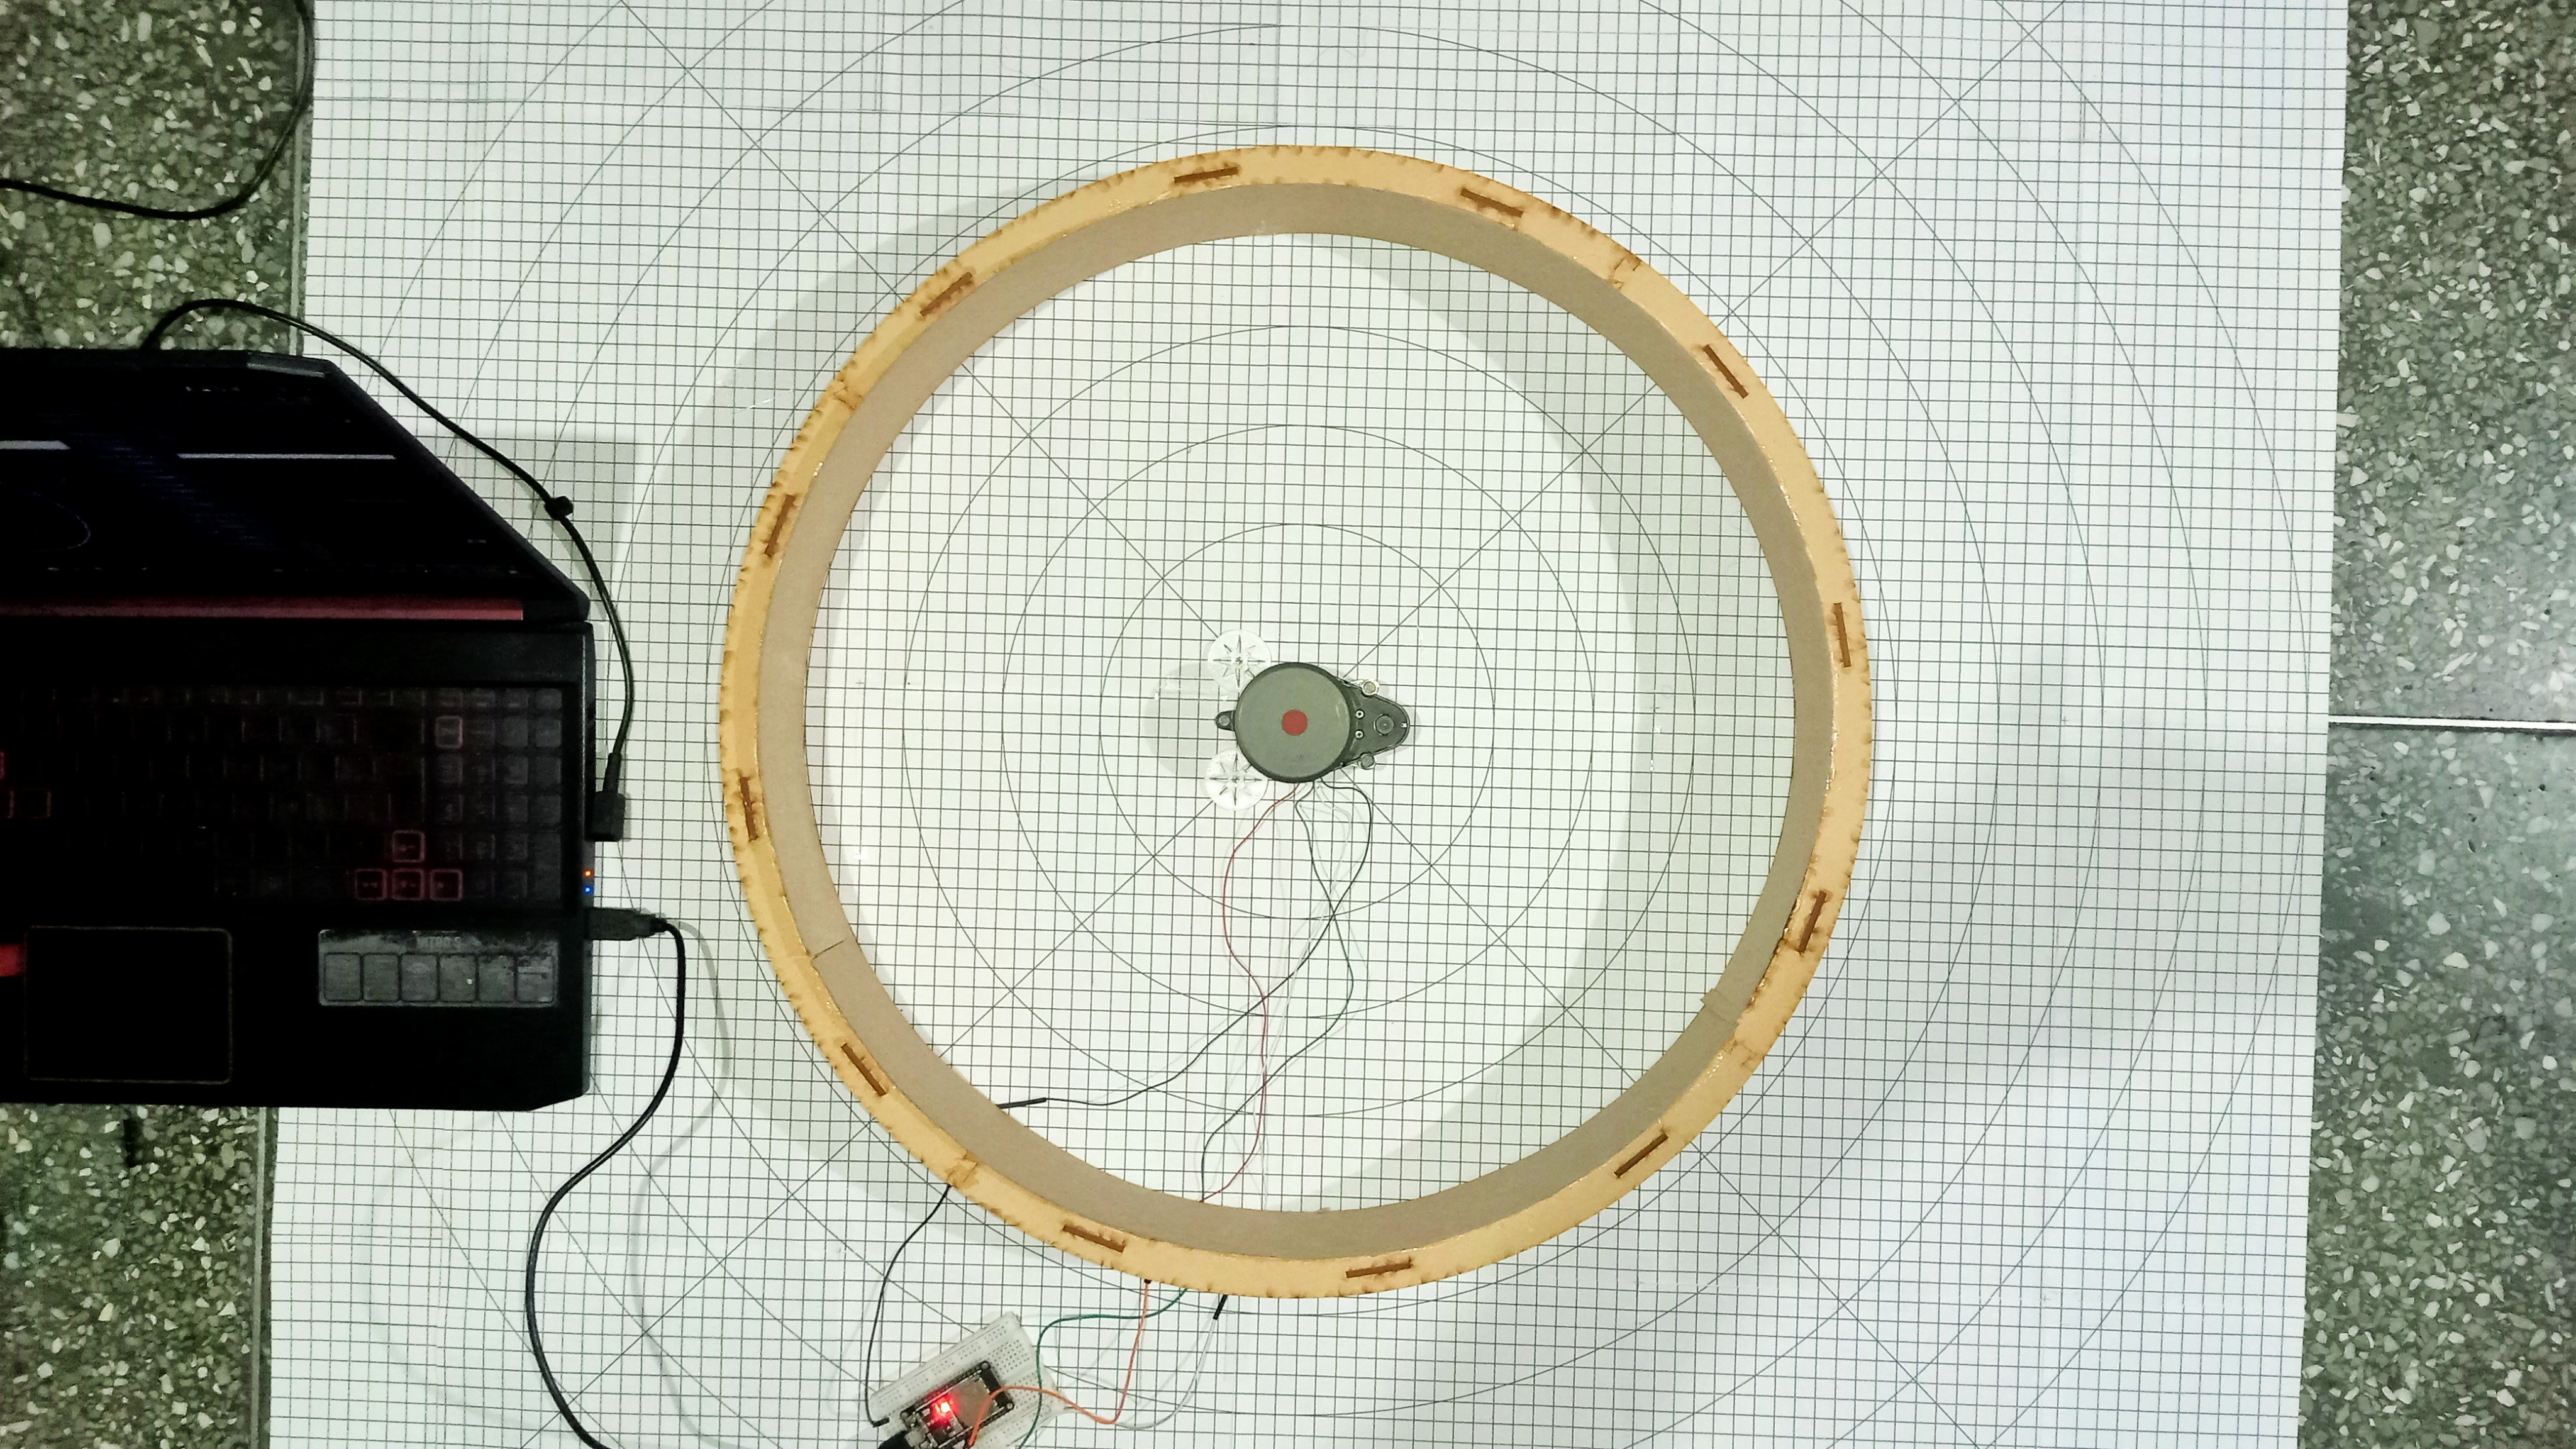
\includegraphics[width=0.6\linewidth]{disposicion_lidar_var_dist3.jpg}}
		\caption{Disposición del sensor FHL-LD20 dentro del entorno circular: 249 mm de radio}
		\label{fig:disposicion_lidar_var3}
		\vspace{1em}
	\end{subfigure}
	\begin{subfigure}{0.45\textwidth}
		\centering
		\includegraphics[width=0.8\linewidth]{0.249m_radius.png}
		\caption{Reconstrucción en coordenadas polares de entorno circular: 249 mm de radio}
		\label{fig:249m_radius_xy}
	\end{subfigure}
	\hspace{1em}
	\begin{subfigure}{0.45\textwidth}
		\centering
		\includegraphics[width=0.83\linewidth]{0.249m_radius_XY.png}
		\caption{Reconstrucción en coordenadas cartesianas de entorno circular: 249 mm de radio}
		\label{fig:249m_radius}
	\end{subfigure}
	\caption{Reconstrucción del entorno circular de 249 mm de radio con 180 revoluciones completas capturadas.}
	\label{fig:disposicion_lidar_var_dist3}
\end{figure}

\begin{figure}[H]
	\centering
	\begin{subfigure}{\textwidth}
		\centering
		\makebox[\textwidth]{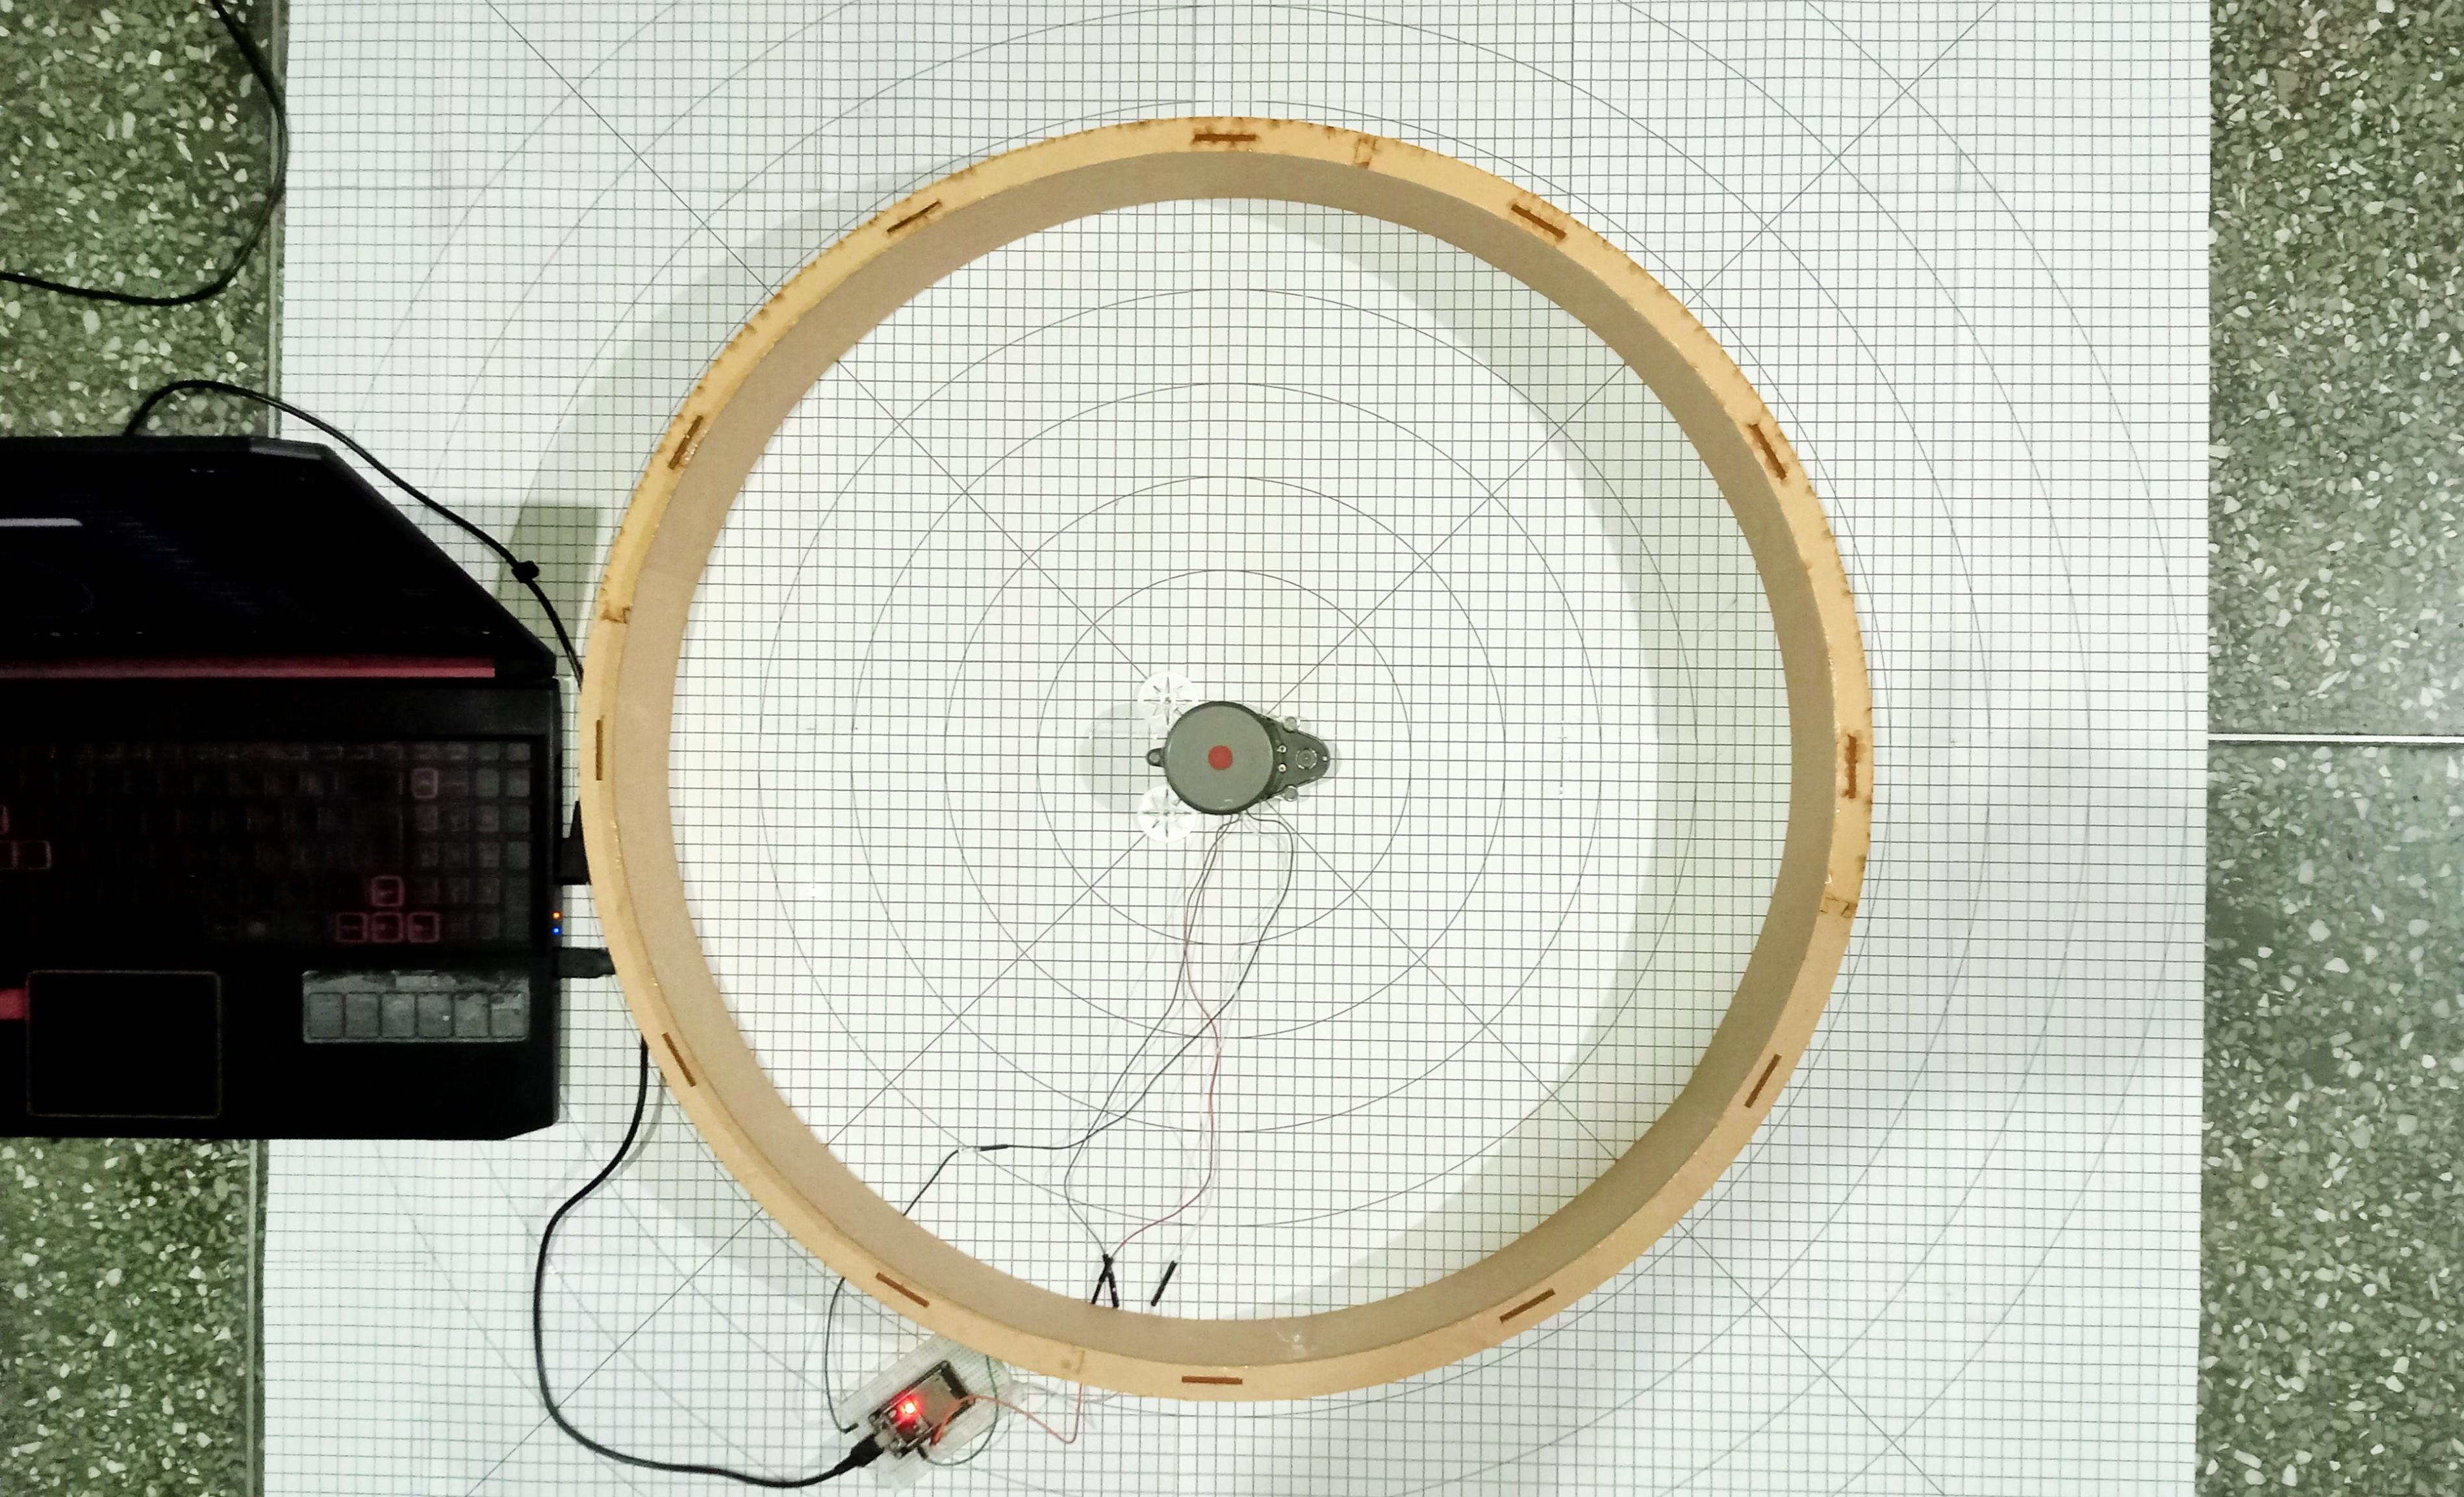
\includegraphics[width=0.6\linewidth]{disposicion_lidar_var_dist4.jpg}}
		\caption{Disposición del sensor FHL-LD20 dentro del entorno circular: 299 mm de radio}
		\label{fig:disposicion_lidar_var4}
		\vspace{1em}
	\end{subfigure}
	\begin{subfigure}{0.45\textwidth}
		\centering
		\includegraphics[width=0.8\linewidth]{0.299m_radius.png}
		\caption{Reconstrucción en coordenadas polares de entorno circular: 299 mm de radio}
		\label{fig:299m_radius_xy}
	\end{subfigure}
	\hspace{1em}
	\begin{subfigure}{0.45\textwidth}
		\centering
		\includegraphics[width=0.83\linewidth]{0.299m_radius_XY.png}
		\caption{Reconstrucción en coordenadas cartesianas de entorno circular: 299 mm de radio}
		\label{fig:299m_radius}
	\end{subfigure}
	\caption{Reconstrucción del entorno circular de 299 mm de radio con 180 revoluciones completas capturadas.}
	\label{fig:disposicion_lidar_var_dist4}
\end{figure}

\begin{figure}[H]
	\centering
	\begin{subfigure}{\textwidth}
		\centering
		\makebox[\textwidth]{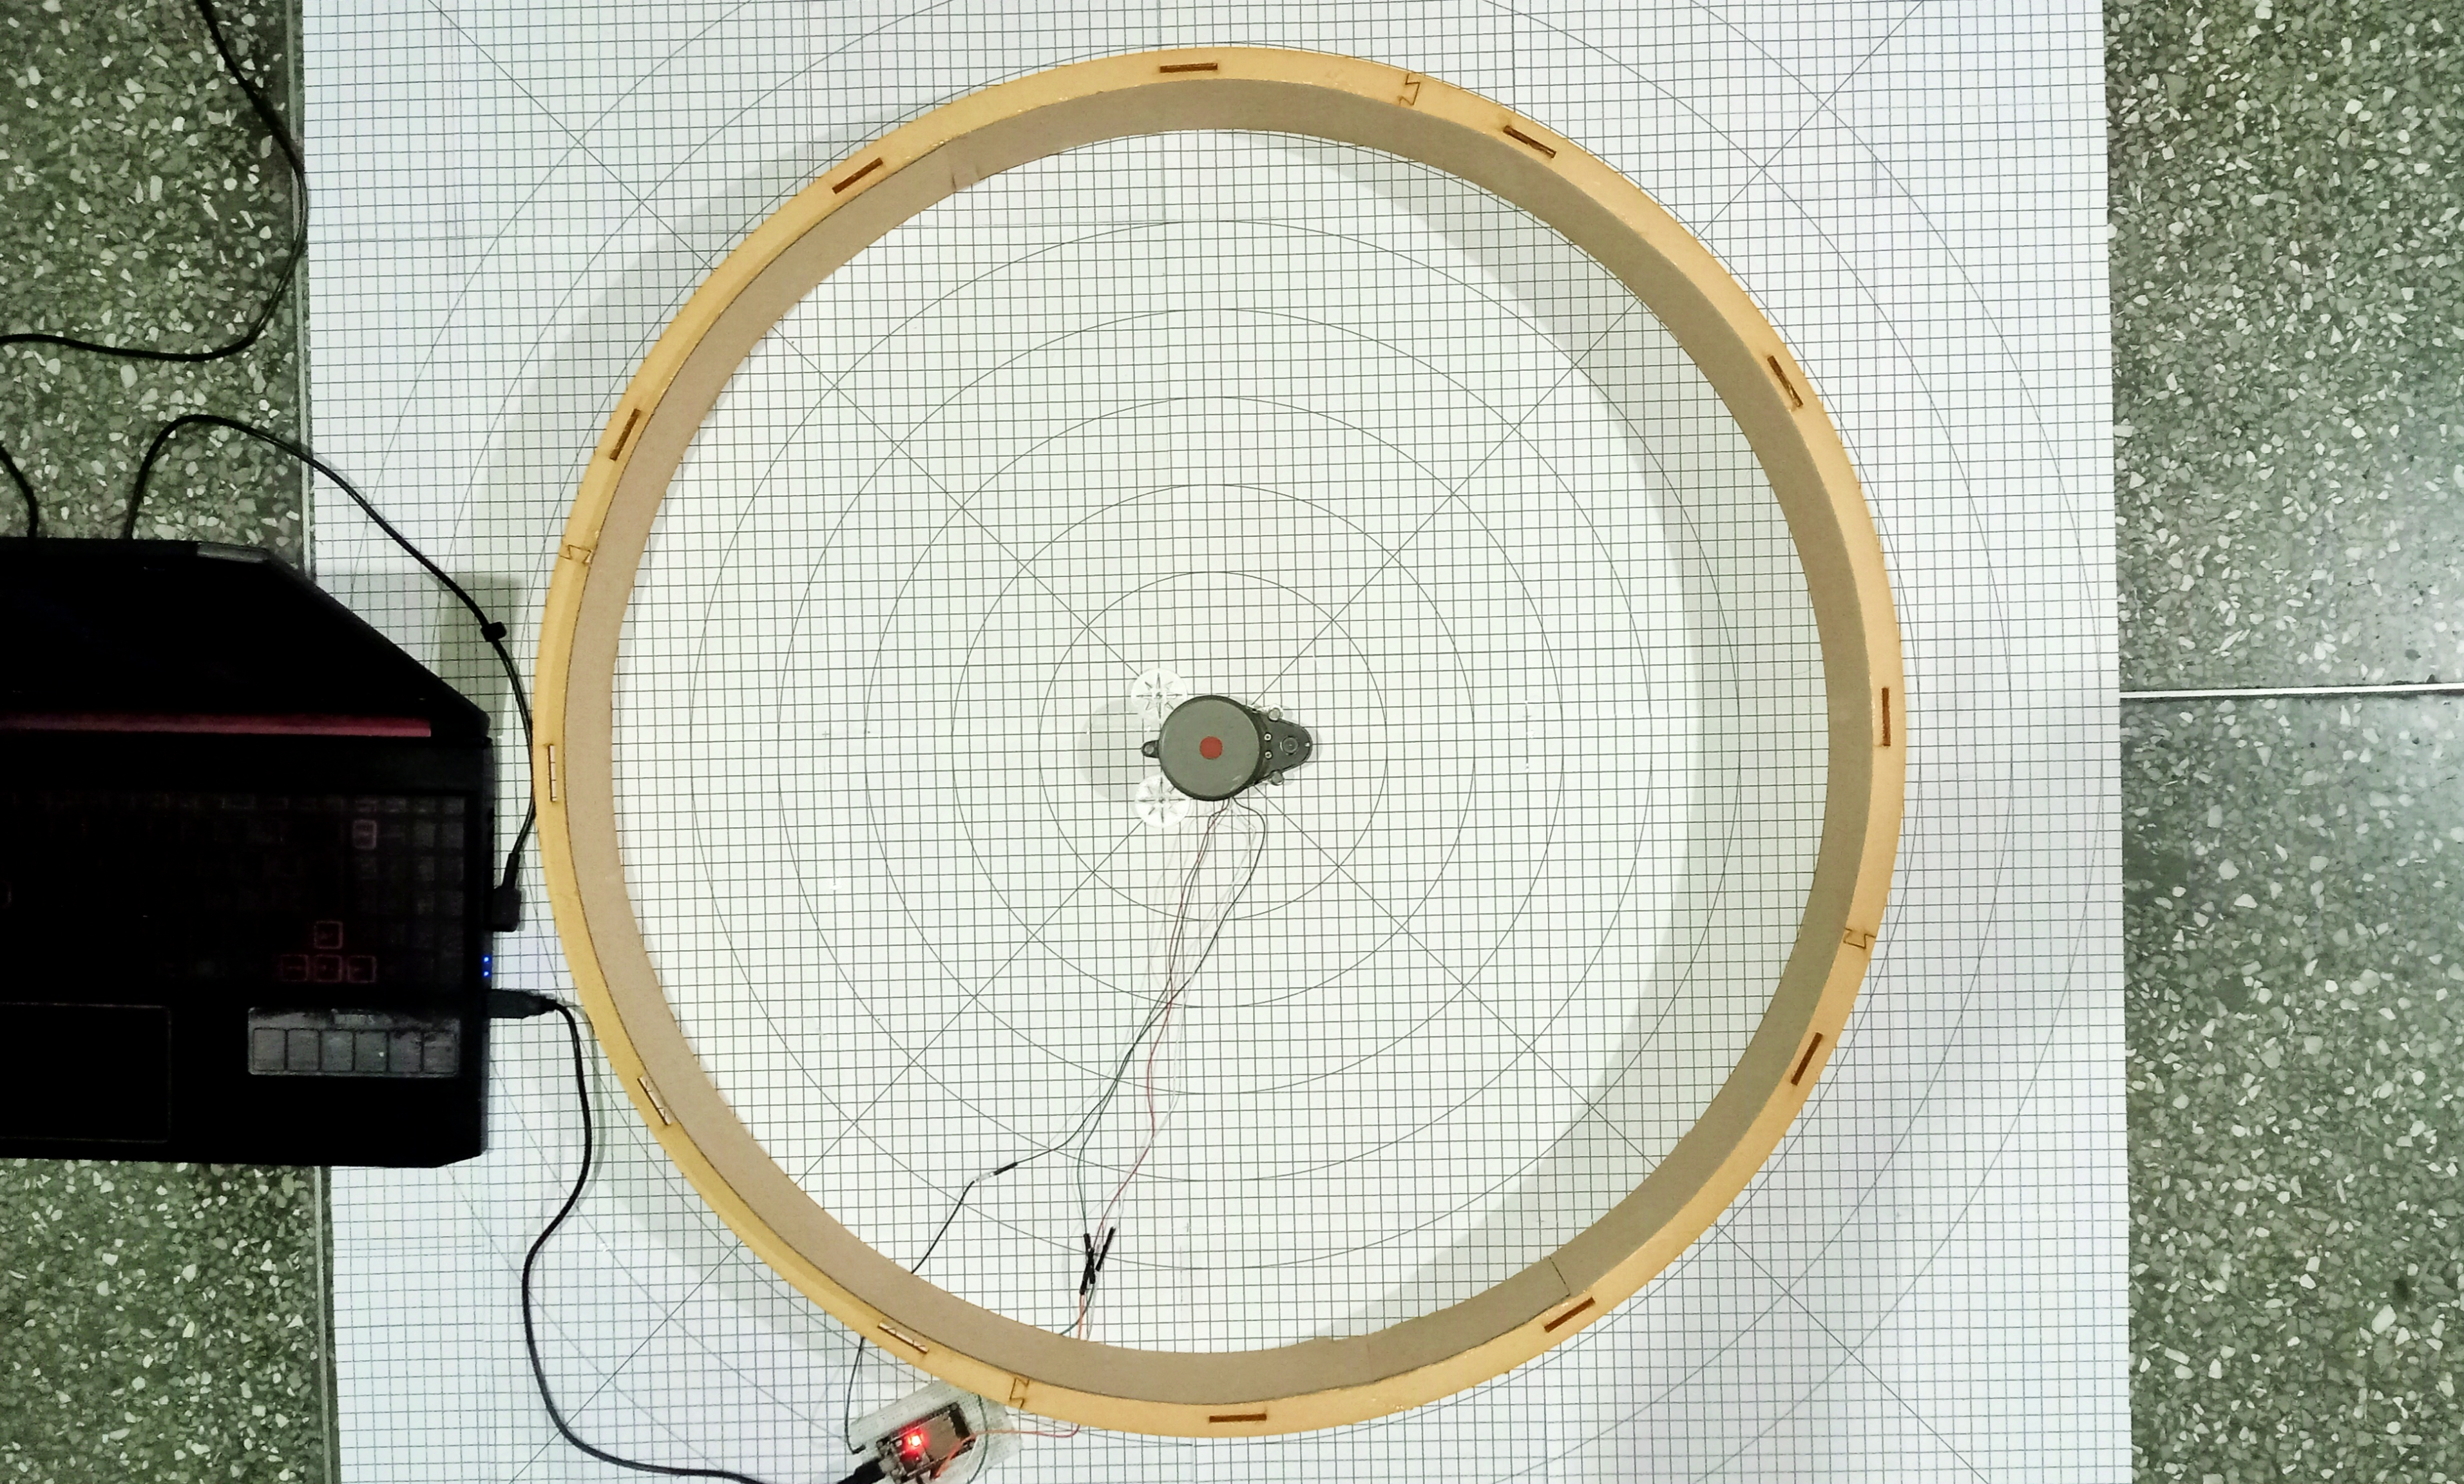
\includegraphics[width=0.6\linewidth]{disposicion_lidar_var_dist5.jpg}}
		\caption{Disposición del sensor FHL-LD20 dentro del entorno circular: 349 mm de radio}
		\label{fig:disposicion_lidar_var5}
		\vspace{1em}
	\end{subfigure}
	\begin{subfigure}{0.45\textwidth}
		\centering
		\includegraphics[width=0.8\linewidth]{0.349m_radius.png}
		\caption{Reconstrucción en coordenadas polares de entorno circular: 349 mm de radio}
		\label{fig:349m_radius_xy}
	\end{subfigure}
	\hspace{1em}
	\begin{subfigure}{0.45\textwidth}
		\centering
		\includegraphics[width=0.83\linewidth]{0.349m_radius_XY.png}
		\caption{Reconstrucción en coordenadas cartesianas de entorno circular: 349 mm de radio}
		\label{fig:349m_radius}
	\end{subfigure}
	\caption{Reconstrucción del entorno circular de 349 mm de radio con 180 revoluciones completas capturadas.}
	\label{fig:disposicion_lidar_var_dist5}
\end{figure}

\begin{figure}[H]
	\centering
	\begin{subfigure}{\textwidth}
		\centering
		\makebox[\textwidth]{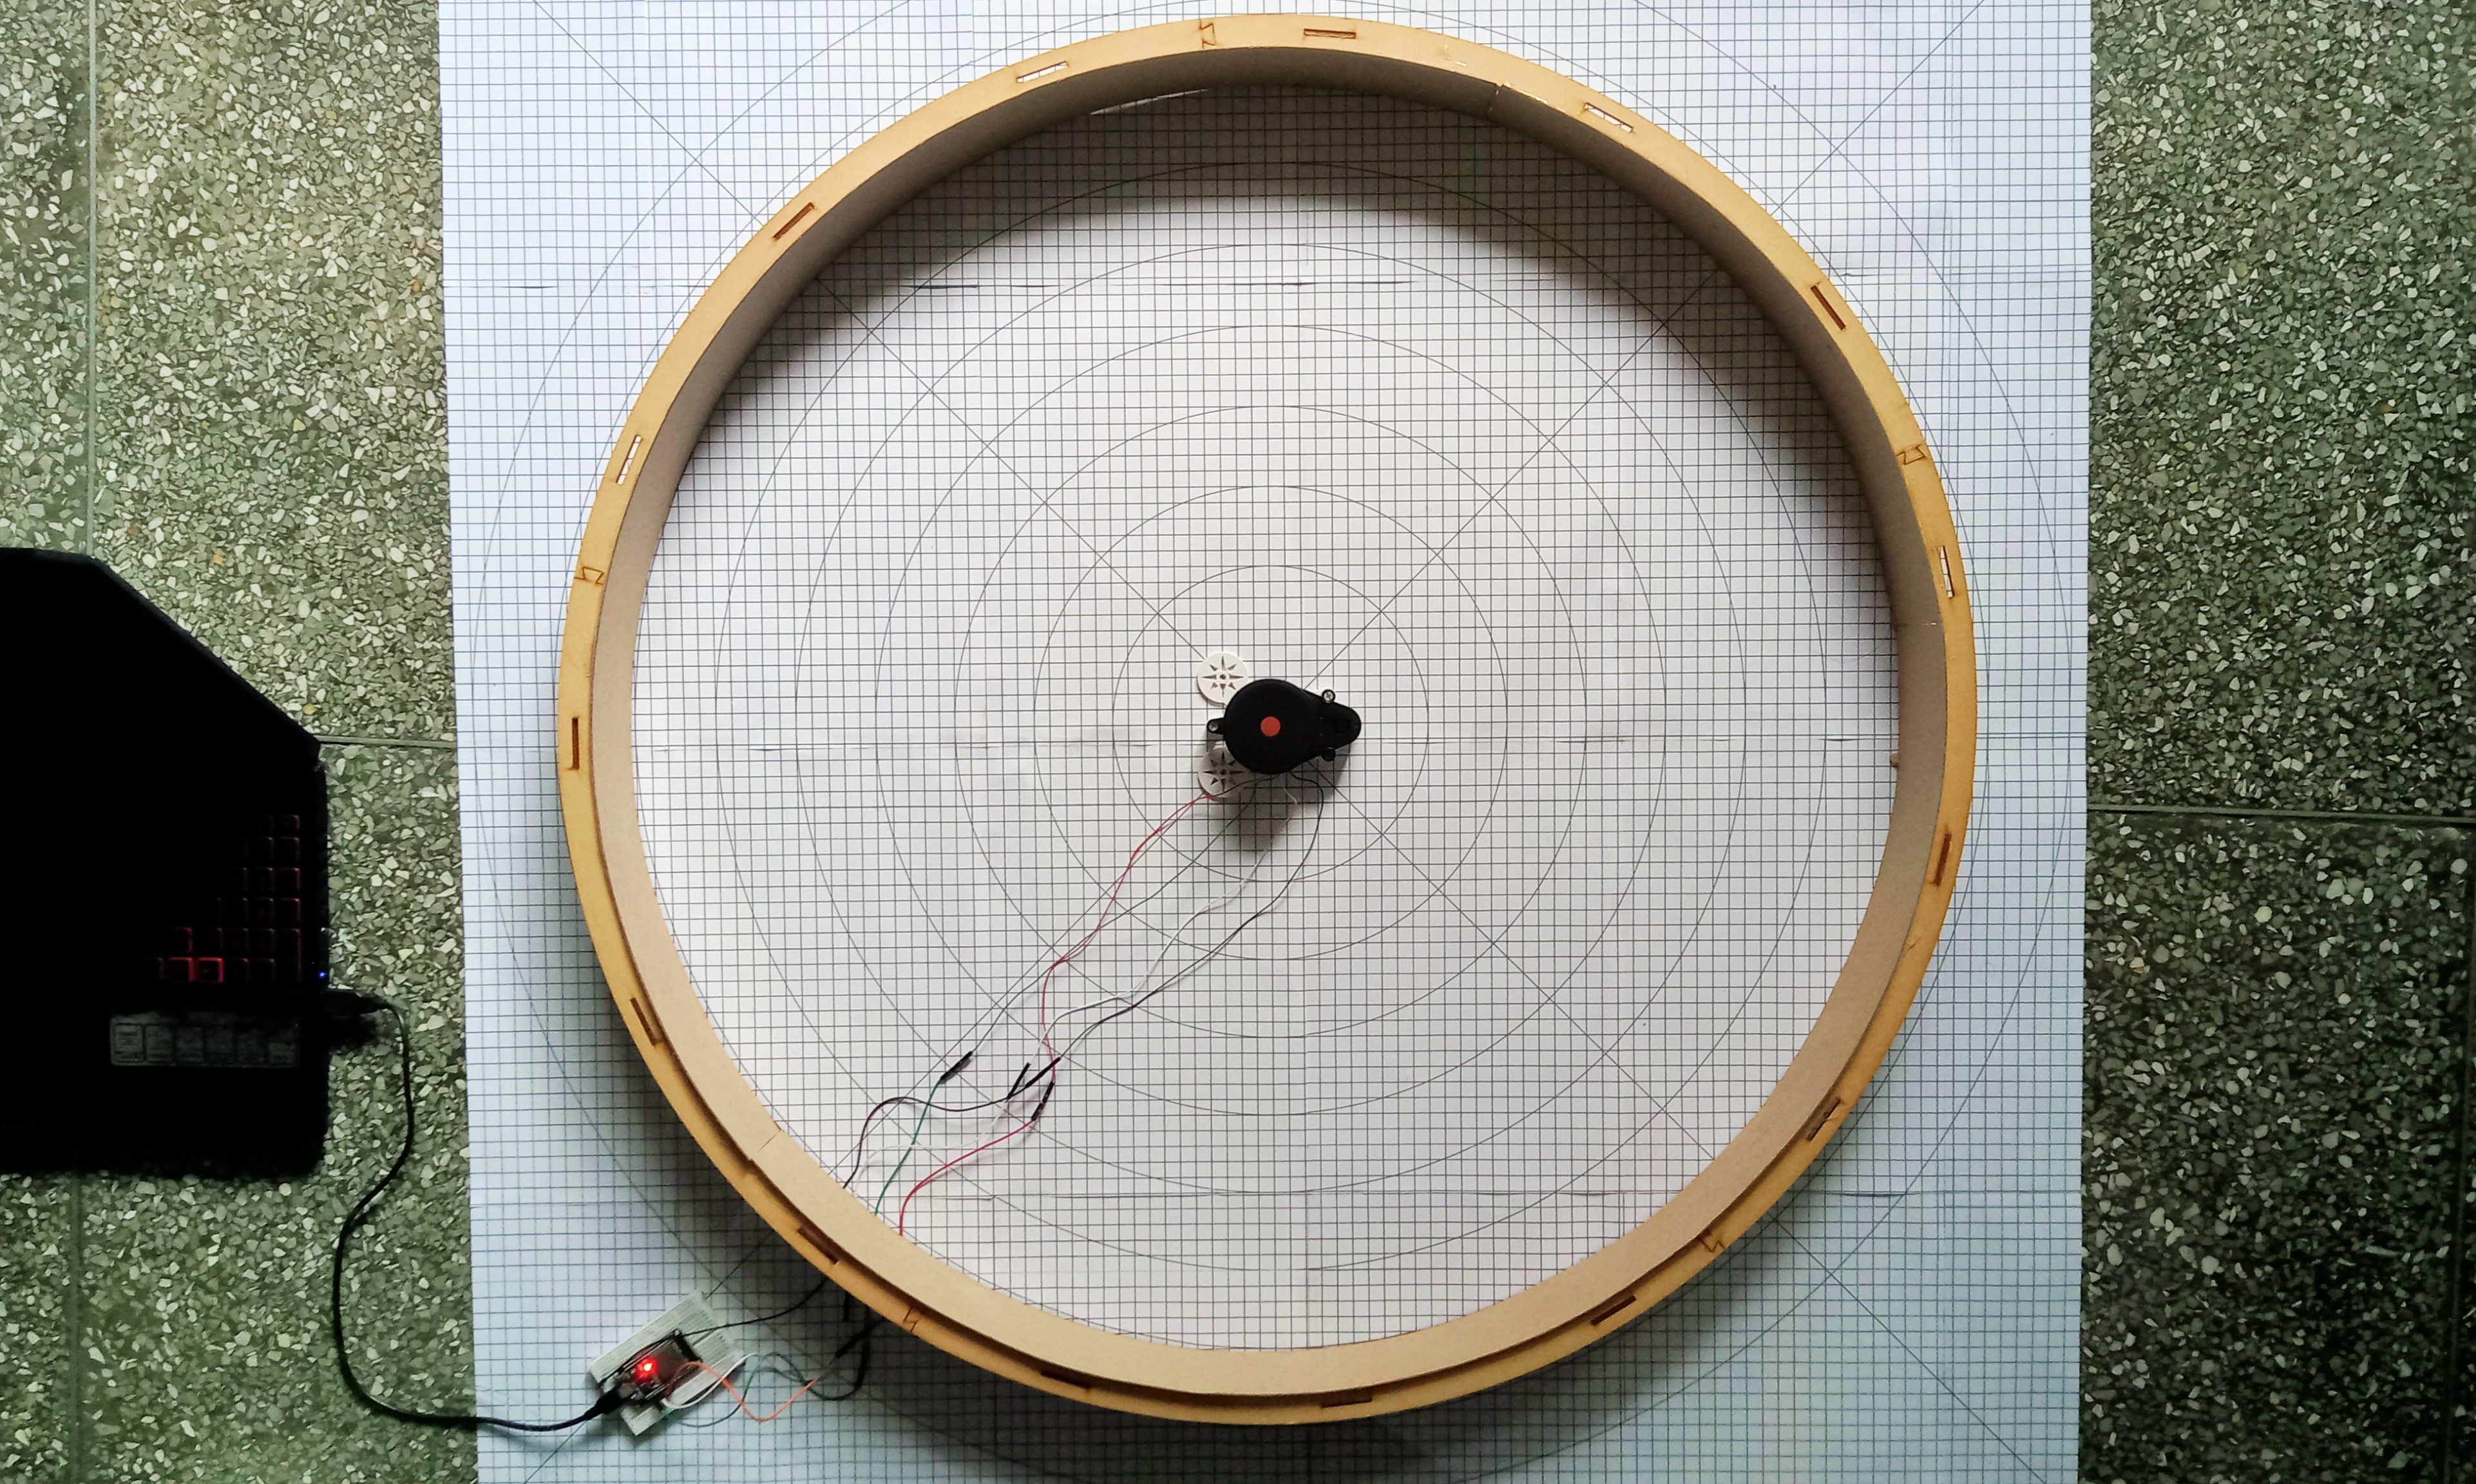
\includegraphics[width=0.6\linewidth]{disposicion_lidar_var_dist6.jpg}}
		\caption{Disposición del sensor FHL-LD20 dentro del entorno circular: 399 mm de radio}
		\label{fig:disposicion_lidar_var6}
		\vspace{1em}
	\end{subfigure}
	\begin{subfigure}{0.45\textwidth}
		\centering
		\includegraphics[width=0.8\linewidth]{0.399m_radius.png}
		\caption{Reconstrucción en coordenadas polares de entorno circular: 399 mm de radio}
		\label{fig:399m_radius_xy}
	\end{subfigure}
	\hspace{1em}
	\begin{subfigure}{0.45\textwidth}
		\centering
		\includegraphics[width=0.83\linewidth]{0.399m_radius_XY.png}
		\caption{Reconstrucción en coordenadas cartesianas de entorno circular: 399 mm de radio}
		\label{fig:399m_radius}
	\end{subfigure}
	\caption{Reconstrucción del entorno circular de 399 mm de radio con 180 revoluciones completas capturadas.}
	\label{fig:disposicion_lidar_var_dist6}
\end{figure}

\begin{figure}[H]
	\centering
	\begin{subfigure}{\textwidth}
		\centering
		\makebox[\textwidth]{\includegraphics[width=0.6\linewidth]{disposicion_lidar_var_dist7.jpg}}
		\caption{Disposición del sensor FHL-LD20 dentro del entorno circular: 449 mm de radio}
		\label{fig:disposicion_lidar_var7}
		\vspace{1em}
	\end{subfigure}
	\begin{subfigure}{0.45\textwidth}
		\centering
		\includegraphics[width=0.8\linewidth]{0.449m_radius.png}
		\caption{Reconstrucción en coordenadas polares de entorno circular: 449 mm de radio}
		\label{fig:449m_radius_xy}
	\end{subfigure}
	\hspace{1em}
	\begin{subfigure}{0.45\textwidth}
		\centering
		\includegraphics[width=0.83\linewidth]{0.449m_radius_XY.png}
		\caption{Reconstrucción en coordenadas cartesianas de entorno circular: 449 mm de radio}
		\label{fig:449m_radius}
	\end{subfigure}
	\caption{Reconstrucción del entorno circular de 449 mm de radio con 180 revoluciones completas capturadas.}
	\label{fig:disposicion_lidar_var_dist7}
\end{figure}

\begin{figure}[H]
	\centering
	\makebox[\textwidth]{\includegraphics[width=1\linewidth]{histograma_dists1}}
	\caption{Distribución de las mediciones de distancia radial para un círculo de 149 mm de radio.}
	\label{fig:histograma_dists1}
\end{figure}

\begin{figure}[H]
	\centering
	\makebox[\textwidth]{\includegraphics[width=1\linewidth]{histograma_dists2}}
	\caption{Distribución de las mediciones de distancia radial para un círculo de 199 mm de radio.}
	\label{fig:histograma_dists2}
\end{figure}

\begin{figure}[H]
	\centering
	\makebox[\textwidth]{\includegraphics[width=1\linewidth]{histograma_dists3}}
	\caption{Distribución de las mediciones de distancia radial para un círculo de 249 mm de radio.}
	\label{fig:histograma_dists3}
\end{figure}

\begin{figure}[H]
	\centering
	\makebox[\textwidth]{\includegraphics[width=1\linewidth]{histograma_dists4}}
	\caption{Distribución de las mediciones de distancia radial para un círculo de 299 mm de radio.}
	\label{fig:histograma_dists4}
\end{figure}

\begin{figure}[H]
	\centering
	\makebox[\textwidth]{\includegraphics[width=1\linewidth]{histograma_dists5}}
	\caption{Distribución de las mediciones de distancia radial para un círculo de 349 mm de radio.}
	\label{fig:histograma_dists5}
\end{figure}

\begin{figure}[H]
	\centering
	\makebox[\textwidth]{\includegraphics[width=1\linewidth]{histograma_dists6}}
	\caption{Distribución de las mediciones de distancia radial para un círculo de 399 mm de radio.}
	\label{fig:histograma_dists6}
\end{figure}

\begin{figure}[H]
	\centering
	\makebox[\textwidth]{\includegraphics[width=1\linewidth]{histograma_dists7}}
	\caption{Distribución de las mediciones de distancia radial para un círculo de 449 mm de radio.}
	\label{fig:histograma_dists7}
\end{figure}

\begin{figure}[H]
	\centering
	\makebox[\textwidth]{\includegraphics[width=1\linewidth]{histograma_dists8}}
	\caption{Distribución de las mediciones de distancia radial para un círculo de 499 mm de radio.}
	\label{fig:histograma_dists8}
\end{figure}

\begin{table}[!ht]
	\centering
	\begin{tabular}{|c|c|c|c|}
		\hline
		\multicolumn{4}{|c|}{\textbf{Radio real de 149 mm}} \\ \hline
		\textbf{No. Prueba} & \textbf{Promedio} & \textbf{Sesgo (\textit{bias})} & \textbf{Varianza muestral} \\ \hline
		1 & 148.9755 & -0.0245 & 0.1036 \\ 
		2 & 148.9741 & -0.0259 & 0.0910 \\ 
		3 & 148.9722 & -0.0278 & 0.0919 \\ 
		4 & 148.9773 & -0.0227 & 0.0917 \\ 
		5 & 148.9755 & -0.0245 & 0.0897 \\ 
		6 & 148.9833 & -0.0167 & 0.0988 \\ 
		7 & 148.9681 & -0.0319 & 0.1199 \\ 
		8 & 148.9722 & -0.0278 & 0.0928 \\ 
		9 & 148.9722 & -0.0278 & 0.0974 \\
		10 & 148.9755 & -0.0245 & 0.0934 \\ \hline
		\textbf{Promedio} & 148.9746 & -0.0254 & 0.0970 \\ \hline
	\end{tabular}
	\caption{Estadísticas de precisión de 180 revoluciones completas de lectura en entorno circular: 149 mm de radio.}
	\label{fig:tabla_dists1}
\end{table}

\begin{table}[H]
	\centering
	\begin{tabular}{|c|c|c|c|}
		\hline
		\multicolumn{4}{|c|}{\textbf{Radio real de 199 mm}} \\ \hline
		\textbf{No. Prueba} & \textbf{Promedio} & \textbf{Sesgo (\textit{bias})} & \textbf{Varianza muestral} \\ \hline
		1 & 199.9338 & 0.9338 & 0.5111 \\ 
		2 & 200.0185 & 1.0185 & 0.4721 \\ 
		3 & 200.0222 & 1.0222 & 0.4766 \\ 
		4 & 200.0264 & 1.0264 & 0.4917 \\ 
		5 & 199.9800 & 0.9880 & 0.4899 \\ 
		6 & 199.9495 & 0.9495 & 0.5222 \\ 
		7 & 199.9477 & 0.9477 & 0.5276 \\ 
		8 & 200.0181 & 1.0181 & 0.4763 \\ 
		9 & 200.0134 & 1.0134 & 0.4811 \\ 
		10 & 199.9769 & 0.9769 & 0.5015 \\ \hline
		\textbf{Promedio} & 199.9887 & 0.9895 & 0.4950 \\ \hline
	\end{tabular}
	\caption{Estadísticas de precisión de 180 revoluciones completas de lectura en entorno circular: 199 mm de radio.}
	\label{fig:tabla_dists2}
\end{table}

\begin{table}[H]
	\centering
	\begin{tabular}{|c|c|c|c|}
		\hline
		\multicolumn{4}{|c|}{\textbf{Radio real de 249 mm}} \\ \hline
		\textbf{No. Prueba} & \textbf{Promedio} & \textbf{Sesgo (\textit{bias})} & \textbf{Varianza muestral} \\ \hline
		1 & 249.1662 & 0.1662 & 0.5425 \\ 
		2 & 249.1361 & 0.1361 & 0.5614 \\ 
		3 & 249.2148 & 0.2148 & 0.5328 \\ 
		4 & 249.2144 & 0.2144 & 0.5446 \\ 
		5 & 249.1366 & 0.1366 & 0.5598 \\ 
		6 & 249.2093 & 0.2093 & 0.5463 \\ 
		7 & 249.1731 & 0.1731 & 0.5453 \\ 
		8 & 249.1764 & 0.1764 & 0.5465 \\ 
		9 & 249.1694 & 0.1694 & 0.5586 \\ 
		10 & 249.1458 & 0.1458 & 0.5554 \\ \hline
		\textbf{Promedio} & 249.1742 & 0.1742 & 0.5493 \\ \hline
	\end{tabular}
	\caption{Estadísticas de precisión de 180 revoluciones completas de lectura en entorno circular: 249 mm de radio.}
	\label{fig:tabla_dists3}
\end{table}

\begin{table}[H]
	\centering
	\begin{tabular}{|c|c|c|c|}
		\hline
		\multicolumn{4}{|c|}{\textbf{Radio real de 299 mm}} \\ \hline
		\textbf{No. Prueba} & \textbf{Promedio} & \textbf{Sesgo (\textit{bias})} & \textbf{Varianza muestral} \\ \hline
		1 & 298.0972 & -0.9028 & 0.5714 \\ 
		2 & 298.0444 & -0.9556 & 0.5047 \\ 
		3 & 297.9861 & -1.0139 & 0.5640 \\ 
		4 & 298.0319 & -0.9681 & 0.5136 \\ 
		5 & 297.9782 & -1.0218 & 0.5549 \\ 
		6 & 298.0449 & -0.9551 & 0.5218 \\ 
		7 & 298.0630 & -0.9370 & 0.5324 \\ 
		8 & 298.0125 & -0.9875 & 0.5135 \\ 
		9 & 298.0000 & -1.0000 & 0.5419 \\ 
		10 & 298.0852 & -0.9148 & 0.5421 \\ \hline
		\textbf{Promedio} & 298.0343 & -0.9657 & 0.5360 \\ \hline
	\end{tabular}
	\caption{Estadísticas de precisión de 180 revoluciones completas de lectura en entorno circular: 299 mm de radio.}
	\label{fig:tabla_dists4}
\end{table}

\begin{table}[H]
	\centering
	\begin{tabular}{|c|c|c|c|}
		\hline
		\multicolumn{4}{|c|}{\textbf{Radio real de 349 mm}} \\ \hline
		\textbf{No. Prueba} & \textbf{Promedio} & \textbf{Sesgo (\textit{bias})} & \textbf{Varianza muestral} \\ \hline
		1 & 348.0944 & -0.9056 & 1.0962 \\ 
		2 & 348.0157 & -0.9843 & 1.0993 \\ 
		3 & 348.0731 & -0.9269 & 1.0887 \\ 
		4 & 348.0000 & -1.0000 & 1.1394 \\ 
		5 & 348.0069 & -0.9931 & 0.9416 \\ 
		6 & 348.1116 & -0.8884 & 1.0552 \\ 
		7 & 348.0403 & -0.9597 & 0.9572 \\ 
		8 & 348.0088 & -0.9912 & 0.9731 \\ 
		9 & 348.0361 & -0.9639 & 0.9380 \\ 
		10 & 347.9569 & -1.0431 & 1.0278 \\ \hline
		\textbf{Promedio} & 348.0344 & -0.9656 & 1.0317 \\ \hline
	\end{tabular}
	\caption{Estadísticas de precisión de 180 revoluciones completas de lectura en entorno circular: 349 mm de radio.}
	\label{fig:tabla_dists5}
\end{table}

\begin{table}[H]
	\centering
	\begin{tabular}{|c|c|c|c|}
		\hline
		\multicolumn{4}{|c|}{\textbf{Radio real de 399 mm}} \\ \hline
		\textbf{No. Prueba} & \textbf{Promedio} & \textbf{Sesgo (\textit{bias})} & \textbf{Varianza muestral} \\ \hline
		1 & 398.4819 & -0.5181 & 1.2132 \\ 
		2 & 398.4778 & -0.5222 & 1.3566 \\ 
		3 & 398.3356 & -0.6644 & 1.3356 \\ 
		4 & 398.4667 & -0.5333 & 1.3940 \\ 
		5 & 398.4019 & -0.5981 & 1.3530 \\ 
		6 & 398.4532 & -0.5468 & 1.3744 \\ 
		7 & 398.3153 & -0.6847 & 1.3730 \\ 
		8 & 398.3764 & -0.6236 & 1.3696 \\ 
		9 & 398.3093 & -0.6907 & 1.3781 \\ 
		10 & 398.3347 & -0.6653 & 1.3817 \\ \hline
		\textbf{Promedio} & 398.3953 & -0.6047 & 1.3529 \\ \hline
	\end{tabular}
	\caption{Estadísticas de precisión de 180 revoluciones completas de lectura en entorno circular: 399 mm de radio.}
	\label{fig:tabla_dists6}
\end{table}

\begin{table}[H]
	\centering
	\begin{tabular}{|c|c|c|c|}
		\hline
		\multicolumn{4}{|c|}{\textbf{Radio real de 449 mm}} \\ \hline
		\textbf{No. Prueba} & \textbf{Promedio} & \textbf{Sesgo (\textit{bias})} & \textbf{Varianza muestral} \\ \hline
		1 & 448.5236 & -0.4764 & 1.5177 \\ 
		2 & 448.5278 & -0.4722 & 1.4258 \\ 
		3 & 448.6005 & -0.3995 & 1.4647 \\ 
		4 & 448.6056 & -0.3944 & 1.4571 \\ 
		5 & 448.5981 & -0.4019 & 1.4642 \\ 
		6 & 448.5574 & -0.4426 & 1.5270 \\ 
		7 & 448.6014 & -0.3986 & 1.5108 \\ 
		8 & 448.5773 & -0.4227 & 1.3936 \\ 
		9 & 448.5181 & -0.4819 & 1.4466 \\
		10 & 448.5847 & -0.4153 & 1.4741 \\ \hline
		\textbf{Promedio} & 448.5695 & -0.4306 & 1.4682 \\ \hline
	\end{tabular}
	\caption{Estadísticas de precisión de 180 revoluciones completas de lectura en entorno circular: 449 mm de radio.}
	\label{fig:tabla_dists7}
\end{table}

\begin{table}[H]
	\centering
	\begin{tabular}{|c|c|c|c|}
		\hline
		\multicolumn{4}{|c|}{\textbf{Radio real de 499 mm}} \\ \hline
		\textbf{No. Prueba} & \textbf{Promedio} & \textbf{Sesgo (\textit{bias})} & \textbf{Varianza muestral} \\ \hline
		1 & 499.3449 & -0.6551 & 2.6114 \\ 
		2 & 499.1468 & -0.8532 & 2.5134 \\ 
		3 & 499.1245 & -0.8755 & 2.5269 \\ 
		4 & 499.2083 & -0.7917 & 2.3679 \\ 
		5 & 499.1384 & -0.8616 & 2.4510 \\ 
		6 & 499.2972 & -0.7028 & 2.4785 \\ 
		7 & 499.2190 & -0.7810 & 2.3240 \\ 
		8 & 499.2046 & -0.7954 & 2.3981 \\ 
		9 & 499.1977 & -0.8023 & 2.3949 \\ 
		10 & 499.2685 & -0.7315 & 2.4364 \\ \hline
		\textbf{Promedio} & 499.2150 & -0.7850 & 2.4503 \\ \hline
	\end{tabular}
	\caption{Estadísticas de precisión de 180 revoluciones completas de lectura en entorno circular: 499 mm de radio.}
	\label{fig:tabla_dists8}
\end{table}
